\documentclass[]{article}

\usepackage[left=2.00cm, right=2.00cm, top=2.00cm, bottom=2.00cm]{geometry}
\usepackage[spanish,es-noshorthands]{babel}
\usepackage[utf8]{inputenc} % para tildes y ñ
\usepackage{graphicx} % para las figuras
\usepackage{xcolor}
\usepackage{listings} % para el código fuente en c++

\lstdefinestyle{customc}{
  belowcaptionskip=1\baselineskip,
  breaklines=true,
  frame=single,
  xleftmargin=\parindent,
  language=C++,
  showstringspaces=false,
  basicstyle=\footnotesize\ttfamily,
  keywordstyle=\bfseries\color{green!40!black},
  commentstyle=\itshape\color{gray!40!gray},
  identifierstyle=\color{black},
  stringstyle=\color{orange},
}
\lstset{style=customc}


%opening
\title{Práctica 2. Programación dinámica}
\author{Juan Carlos Lucena Monje \\ % mantenga las dos barras al final de la línea y este comentario
juancarlos.lucenamonje@alum.uca.es \\ % mantenga las dos barras al final de la línea y este comentario
Teléfono: 637929532 \\ % mantenga las dos barras al final de la linea y este comentario
NIF: 45899713q \\ % mantenga las dos barras al final de la línea y este comentario
}


\begin{document}

\maketitle

%\begin{abstract}
%\end{abstract}

% Ejemplo de ecuación a trozos
%
%$f(i,j)=\left\{ 
%  \begin{array}{lcr}
%      i + j & si & i < j \\ % caso 1
%      i + 7 & si & i = 1 \\ % caso 2
%      2 & si & i \geq j     % caso 3
%  \end{array}
%\right.$

\begin{enumerate}
\item Formalice a continuación y describa la función que asigna un determinado valor a cada uno de los tipos de defensas.

Calculo el valor en funcion de la distancia a la que este de los obstaculos. Utilizo un incrementador para clasificar las distancias, consiguiendo que a mayor distancia haya menos valor tendra.

% Elimine los símbolos de tanto por ciento para descomentar las siguientes instrucciones e incluir una imagen en su respuesta. La mejor ubicación de la imagen será determinada por el compilador de Latex. No tiene por qué situarse a continuación en el fichero en formato pdf resultante.
\begin{figure}
\centering
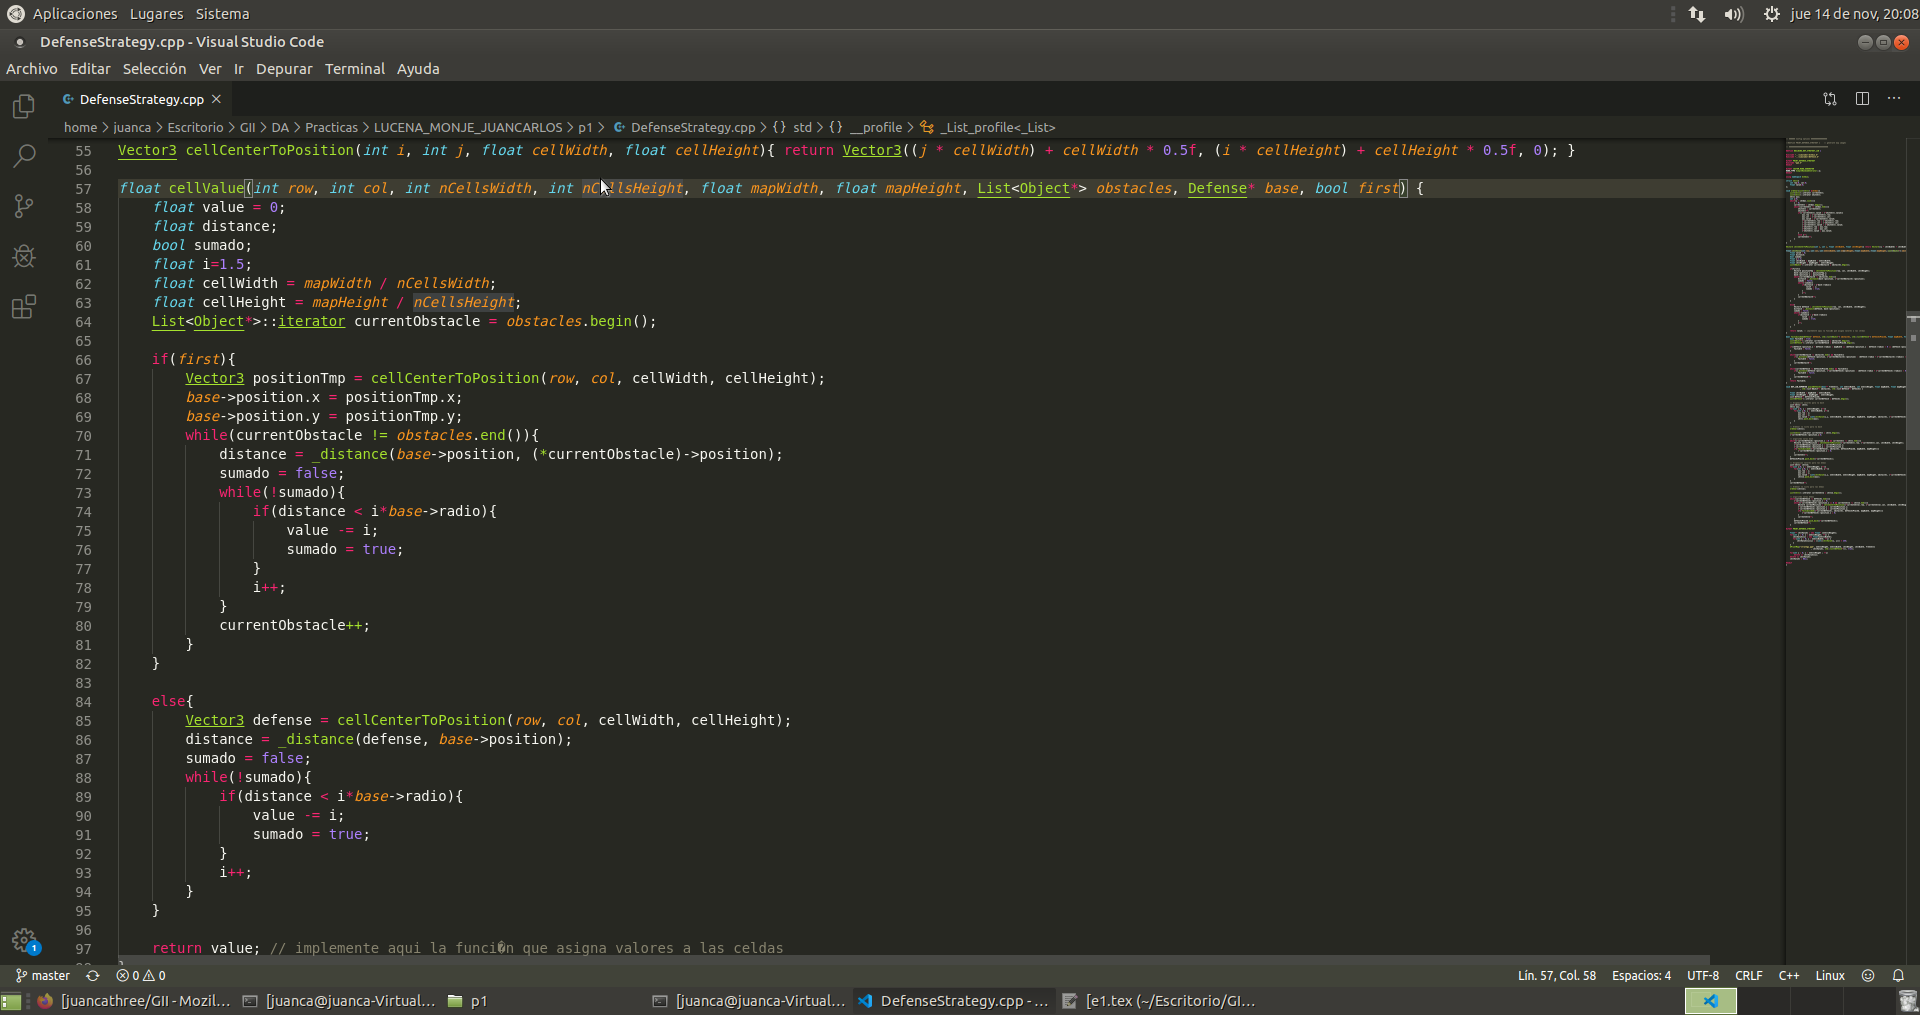
\includegraphics[width=0.7\linewidth]{./defenseValueCellsHead} % no es necesario especificar la extensión del archivo que contiene la imagen
\caption{Estrategia devoradora para la mina}
\label{fig:defenseValueCellsHead}
\end{figure}


\item Describa la estructura o estructuras necesarias para representar la tabla de subproblemas resueltos.

Escriba aquí su respuesta al ejercicio 2.

\item En base a los dos ejercicios anteriores, diseñe un algoritmo que determine el máximo beneficio posible a obtener dada una combinación de defensas y \emph{ases} disponibles. Muestre a continuación el código relevante.

Escriba aquí su respuesta al ejercicio 3.

\item Diseñe un algoritmo que recupere la combinación óptima de defensas a partir del contenido de la tabla de subproblemas resueltos. Muestre a continuación el código relevante.

Una vez haya seleccionado una celda del conjunto si es valida se asigna y ya no puede excluirse y en el caso de que no sea valida no se vuevlve a tener nunca en cuenta.


\end{enumerate}

Todo el material incluido en esta memoria y en los ficheros asociados es de mi autoría o ha sido facilitado por los profesores de la asignatura. Haciendo entrega de este documento confirmo que he leído la normativa de la asignatura, incluido el punto que respecta al uso de material no original.

\end{document}
